\documentclass[10pt]{article}
\usepackage{tmlr}

% --- Core Math & Typography Packages ---
\usepackage{amsmath,amssymb,amsfonts,amsthm}
\usepackage{mathtools}
\usepackage{microtype}
\usepackage{booktabs}
\usepackage{multirow}
\usepackage{array}
\usepackage{graphicx}
\usepackage{xcolor}
\usepackage{enumitem}
\usepackage{pifont}
\usepackage{url}
\usepackage[colorlinks=true,linkcolor=blue!80!black,citecolor=blue!80!black,urlcolor=blue!80!black]{hyperref}
\usepackage{natbib}

% --- Table & Paragraph Settings ---
\renewcommand{\arraystretch}{1.12}
\setlength{\textfloatsep}{10pt plus 2pt minus 2pt}
\setlength{\floatsep}{8pt plus 2pt minus 2pt}
\setlength{\intextsep}{8pt plus 2pt minus 2pt}

% --- Theorem & Math Helpers ---
\theoremstyle{definition}
\newtheorem{definition}{Definition}
\newtheorem{proposition}{Proposition}

% --- Vertical Spacing: 3x Whitespace on Page 1, Balanced Page Margins & Vertically Centered Footer ---
\setlength{\topmargin}{-0.30in}
\setlength{\headsep}{14pt}
\setlength{\textheight}{9.15in}
\setlength{\footskip}{30pt}
\setlength{\aftertitskip}{20pt}

% --- Formula Spacing: Distinct Space Above & Below Display Equations ---
\setlength{\abovedisplayskip}{12pt plus 3pt minus 2pt}
\setlength{\belowdisplayskip}{12pt plus 3pt minus 2pt}
\setlength{\abovedisplayshortskip}{8pt plus 3pt minus 2pt}
\setlength{\belowdisplayshortskip}{8pt plus 3pt minus 2pt}

% --- Table & Float Spacing: Distinct Space Above & Below Tables & Captions ---
\setlength{\floatsep}{14pt plus 2pt minus 2pt}
\setlength{\textfloatsep}{14pt plus 2pt minus 2pt}
\setlength{\intextsep}{14pt plus 2pt minus 2pt}
\setlength{\abovecaptionskip}{8pt plus 2pt minus 2pt}
\setlength{\belowcaptionskip}{6pt plus 2pt minus 1pt}

\makeatletter
\def\@maketitle{\vbox{\hsize\textwidth
\vskip 14pt
{\LARGE\bfseries \@title\par}\vskip \aftertitskip
\if@accepted
    \if@preprint
        \@startauthor \@author \@endauthor
    \else
        \@startauthor \@author \\ \\ {\bf Reviewed on OpenReview:} \openreview \@endauthor
    \fi
\else
    \@startauthor Anonymous authors\\Paper under double-blind review \@endauthor
\fi
\vskip 20pt}}
\makeatother

% --- Title Block ---
\title{Supplementary Material: CRBench \\ \large A Method-Agnostic, Resource-Aware \\ Evaluation Framework for Long-Context \\ Large Language Models}

\author{\name Anonymous authors \\
        \addr Paper under double-blind review --- Technical Report}

\begin{document}

\maketitle

\appendix

% ==============================================================================
% SECTION A: FULL PER-MODEL LEADERBOARDS
% ==============================================================================
\section{Full Per-Model Leaderboards}
\label{sec:app_leaderboards}

This section provides complete Part~1 (Algorithmic Representation Fidelity $\mathcal{S}_{\text{res}}$) and Part~2 (Hardware System Serving Utility $\mathcal{S}_{\text{sys}}$) leaderboards for all three evaluated foundation model families across 3,150 queries.

\subsection{Gemma 4 E2B Leaderboard (\texorpdfstring{$2\text{K} \to 128\text{K}$}{2K to 128K} Context Ladder, 1,050 Queries)}

\begin{table}[h]
\vspace{6pt}
\centering
\small
\caption{Gemma 4 E2B Part 1 ($\mathcal{S}_{\text{res}}$) Algorithmic Representation Leaderboard.}
\label{tab:e2b_sres}
\begin{tabular}{clcccc}
\toprule
\textbf{Rank} & \textbf{Method} & \textbf{Accuracy} & $b_{\text{eff}}^{\text{agg}}$ & \textbf{VRAM Saved} & $\mathcal{S}_{\text{res}}$ \\
\midrule
1 & \textbf{SnapKV} & 46.8\% & 6.00 bpt & 62.5\% & \textbf{51.5} \\
2 & \textbf{KIVI} & 46.4\% & 6.01 bpt & 62.4\% & 51.2 \\
3 & \textbf{DKV-Mid} & 44.7\% & 5.46 bpt & 65.9\% & 51.0 \\
4 & \textbf{DKV-High} & 46.7\% & 10.78 bpt & 32.6\% & 42.5 \\
5 & \textbf{Low-Rank KV} & 31.2\% & 6.07 bpt & 62.1\% & 40.5 \\
6 & \textbf{StreamingLLM} & 22.9\% & 6.00 bpt & 62.5\% & 34.8 \\
7 & \textbf{Dense FP16} (Reference) & 46.4\% & 16.00 bpt & 0.0\% & 32.5 \\
8 & \textbf{KV-Merging} & 13.3\% & 6.01 bpt & 62.5\% & 28.0 \\
\bottomrule
\end{tabular}
\end{table}

\begin{table}[h]
\vspace{6pt}
\centering
\small
\caption{Gemma 4 E2B Part 2 ($\mathcal{S}_{\text{sys}}$) Hardware System Serving Leaderboard.}
\label{tab:e2b_ssys}
\begin{tabular}{clccccccc}
\toprule
\textbf{Rank} & \textbf{Method} & $\mathcal{S}_{\text{sys}}$ & $\mathcal{S}_{\text{res}}$ & \textbf{TTFT} & \textbf{Decode} & \textbf{Peak VRAM} & $\phi$ \\
\midrule
1 & \textbf{KIVI} & \textbf{64.6} & 51.2 & 12.51s & 11.9 tok/s & 847.0 MB & 0.96$\times$ \\
2 & \textbf{SnapKV} & 60.6 & 51.5 & 13.04s & 12.9 tok/s & 2088.2 MB & 0.82$\times$ \\
3 & \textbf{DKV-Mid} & 59.1 & 51.0 & 22.26s & 13.8 tok/s & 1389.9 MB & 0.78$\times$ \\
4 & \textbf{Low-Rank KV} & 57.4 & 40.5 & 12.80s & 12.3 tok/s & 849.8 MB & 0.97$\times$ \\
5 & \textbf{StreamingLLM} & 54.3 & 34.8 & 12.58s & 13.7 tok/s & 847.4 MB & 1.00$\times$ \\
6 & \textbf{Dense FP16} & 52.8 & 32.5 & 13.18s & 13.4 tok/s & 1118.4 MB & 1.00$\times$ \\
7 & \textbf{DKV-High} & 52.7 & 42.5 & 23.40s & 13.8 tok/s & 1391.0 MB & 0.77$\times$ \\
8 & \textbf{KV-Merging} & 49.6 & 28.0 & 12.59s & 13.7 tok/s & 847.8 MB & 1.00$\times$ \\
\bottomrule
\end{tabular}
\end{table}

\clearpage
\subsection{Gemma 4 E4B Leaderboard (\texorpdfstring{$2\text{K} \to 32\text{K}$}{2K to 32K} Context Ladder, 1,050 Queries)}

\begin{table}[h]
\vspace{6pt}
\centering
\small
\caption{Gemma 4 E4B Part 1 ($\mathcal{S}_{\text{res}}$) Algorithmic Representation Leaderboard.}
\label{tab:e4b_sres}
\begin{tabular}{clcccc}
\toprule
\textbf{Rank} & \textbf{Method} & \textbf{Accuracy} & $b_{\text{eff}}^{\text{agg}}$ & \textbf{VRAM Saved} & $\mathcal{S}_{\text{res}}$ \\
\midrule
1 & \textbf{KIVI} & 62.0\% & 6.04 bpt & 62.2\% & \textbf{62.1} \\
2 & \textbf{SnapKV} & 60.0\% & 6.00 bpt & 62.5\% & 60.8 \\
3 & \textbf{DKV-Mid} & 55.3\% & 5.00 bpt & 68.7\% & 59.4 \\
4 & \textbf{DKV-High} & 61.3\% & 10.68 bpt & 33.3\% & 52.9 \\
5 & \textbf{Low-Rank KV} & 48.8\% & 6.27 bpt & 60.8\% & 52.4 \\
6 & \textbf{Dense FP16} (Reference) & 64.0\% & 16.00 bpt & 0.0\% & 44.8 \\
7 & \textbf{StreamingLLM} & 25.5\% & 6.00 bpt & 62.5\% & 36.6 \\
8 & \textbf{KV-Merging} & 25.3\% & 6.03 bpt & 62.3\% & 36.4 \\
\bottomrule
\end{tabular}
\end{table}

\begin{table}[h]
\vspace{6pt}
\centering
\small
\caption{Gemma 4 E4B Part 2 ($\mathcal{S}_{\text{sys}}$) Hardware System Serving Leaderboard.}
\label{tab:e4b_ssys}
\begin{tabular}{clccccccc}
\toprule
\textbf{Rank} & \textbf{Method} & $\mathcal{S}_{\text{sys}}$ & $\mathcal{S}_{\text{res}}$ & \textbf{TTFT} & \textbf{Decode} & \textbf{Peak VRAM} & $\phi$ \\
\midrule
1 & \textbf{KIVI} & \textbf{73.4} & 62.1 & 2.84s & 12.8 tok/s & 761.3 MB & 1.00$\times$ \\
2 & \textbf{DKV-Mid} & 66.3 & 59.4 & 5.06s & 12.3 tok/s & 760.7 MB & 0.83$\times$ \\
3 & \textbf{Low-Rank KV} & 65.9 & 52.4 & 3.18s & 13.1 tok/s & 761.5 MB & 0.97$\times$ \\
4 & \textbf{Dense FP16} & 61.4 & 44.8 & 2.96s & 12.4 tok/s & 761.5 MB & 1.00$\times$ \\
5 & \textbf{DKV-High} & 60.0 & 52.9 & 6.25s & 12.2 tok/s & 761.0 MB & 0.76$\times$ \\
6 & \textbf{StreamingLLM} & 55.6 & 36.6 & 2.92s & 13.6 tok/s & 761.4 MB & 1.00$\times$ \\
7 & \textbf{KV-Merging} & 55.5 & 36.4 & 2.91s & 13.5 tok/s & 761.5 MB & 1.00$\times$ \\
8 & \textbf{SnapKV} & 48.6 & 60.8 & 83.38s & 10.6 tok/s & 2632.4 MB & 0.20$\times$ \\
\bottomrule
\end{tabular}
\end{table}

\clearpage
\subsection{Qwen2.5 7B Leaderboard (\texorpdfstring{$2\text{K} \to 32\text{K}$}{2K to 32K} Context Ladder, 1,050 Queries)}

\begin{table}[h]
\vspace{6pt}
\centering
\small
\caption{Qwen2.5 7B Part 1 ($\mathcal{S}_{\text{res}}$) Algorithmic Representation Leaderboard.}
\label{tab:q7b_sres}
\begin{tabular}{clcccc}
\toprule
\textbf{Rank} & \textbf{Method} & \textbf{Accuracy} & $b_{\text{eff}}^{\text{agg}}$ & \textbf{VRAM Saved} & $\mathcal{S}_{\text{res}}$ \\
\midrule
1 & \textbf{KV-Quant} & 60.7\% & 6.04 bpt & 62.2\% & \textbf{61.1} \\
2 & \textbf{SnapKV} & 58.2\% & 6.00 bpt & 62.5\% & 59.5 \\
3 & \textbf{DKV-Mid} & 53.3\% & 5.84 bpt & 63.5\% & 56.3 \\
4 & \textbf{DKV-High} & 59.1\% & 12.14 bpt & 24.1\% & 48.6 \\
5 & \textbf{StreamingLLM} & 36.5\% & 6.00 bpt & 62.5\% & 44.3 \\
6 & \textbf{Dense FP16} (Reference) & 60.0\% & 16.00 bpt & 0.0\% & 42.0 \\
7 & \textbf{Low-Rank KV} & 28.6\% & 6.09 bpt & 62.0\% & 38.6 \\
8 & \textbf{KV-Merging} & 19.9\% & 6.03 bpt & 62.3\% & 32.6 \\
\bottomrule
\end{tabular}
\end{table}

\begin{table}[h]
\vspace{6pt}
\centering
\small
\caption{Qwen2.5 7B Part 2 ($\mathcal{S}_{\text{sys}}$) Hardware System Serving Leaderboard.}
\label{tab:q7b_ssys}
\begin{tabular}{clccccccc}
\toprule
\textbf{Rank} & \textbf{Method} & $\mathcal{S}_{\text{sys}}$ & $\mathcal{S}_{\text{res}}$ & \textbf{TTFT} & \textbf{Decode} & \textbf{Peak VRAM} & $\phi$ \\
\midrule
1 & \textbf{KV-Quant} & \textbf{72.8} & 61.1 & 5.46s & 16.4 tok/s & 3854.3 MB & 1.00$\times$ \\
2 & \textbf{StreamingLLM} & 61.0 & 44.3 & 5.51s & 24.9 tok/s & 3854.4 MB & 1.00$\times$ \\
3 & \textbf{Dense FP16} & 59.4 & 42.0 & 5.56s & 16.3 tok/s & 3854.2 MB & 1.00$\times$ \\
4 & \textbf{Low-Rank KV} & 54.9 & 38.6 & 6.82s & 18.1 tok/s & 3854.4 MB & 0.93$\times$ \\
5 & \textbf{DKV-Mid} & 54.2 & 56.3 & 39.55s & 15.3 tok/s & 3854.2 MB & 0.49$\times$ \\
6 & \textbf{SnapKV} & 53.7 & 59.5 & 58.69s & 22.2 tok/s & 5132.6 MB & 0.40$\times$ \\
7 & \textbf{KV-Merging} & 52.8 & 32.6 & 5.51s & 25.8 tok/s & 3854.4 MB & 1.00$\times$ \\
8 & \textbf{DKV-High} & 48.5 & 48.6 & 41.88s & 15.3 tok/s & 3854.5 MB & 0.48$\times$ \\
\bottomrule
\end{tabular}
\end{table}

\clearpage
% ==============================================================================
% SECTION B: FULL TASK-WISE BREAKDOWN TABLES
% ==============================================================================
\section{Full Task-Wise Breakdown Tables}
\label{sec:app_tasks}

\subsection{Gemma 4 E2B Task Breakdown (5 Tasks \texorpdfstring{$\times$}{x} 5 Context Lengths)}

\begin{table}[h]
\vspace{6pt}
\centering
\small
\caption{Gemma 4 E2B Task-Wise Accuracy Breakdown across Context Lengths (2K to 128K tokens).}
\label{tab:e2b_task_breakdown}
\begin{tabular}{lcccccc}
\toprule
\textbf{Task / Method} & \textbf{2K} & \textbf{8K} & \textbf{32K} & \textbf{64K} & \textbf{128K} & \textbf{Mean Acc} \\
\midrule
\multicolumn{7}{l}{\textbf{Task 1: Single Needle in a Haystack (Single NIAH)}} \\
\textbf{KIVI} & 100.0\% & 100.0\% & 100.0\% & 100.0\% & 100.0\% & \textbf{100.0\%} \\
\textbf{DKV-High} & 100.0\% & 100.0\% & 100.0\% & 100.0\% & 100.0\% & \textbf{100.0\%} \\
\textbf{Dense FP16} & 100.0\% & 100.0\% & 100.0\% & 100.0\% & 100.0\% & \textbf{100.0\%} \\
\textbf{SnapKV} & 91.7\% & 100.0\% & 100.0\% & 100.0\% & 100.0\% & 98.3\% \\
\textbf{DKV-Mid} & 100.0\% & 100.0\% & 100.0\% & 100.0\% & 83.3\% & 96.7\% \\
\textbf{Low-Rank KV} & 100.0\% & 53.3\% & 50.0\% & 50.0\% & 50.0\% & 60.7\% \\
\textbf{StreamingLLM} & 54.9\% & 50.0\% & 50.0\% & 50.0\% & 50.0\% & 51.0\% \\
\textbf{KV-Merging} & 48.7\% & 52.1\% & 42.7\% & 52.4\% & 35.7\% & 46.3\% \\
\midrule
\multicolumn{7}{l}{\textbf{Task 2: Multi-Needle Extraction (Multi NIAH)}} \\
\textbf{DKV-High} & 33.3\% & 33.3\% & 33.3\% & 33.3\% & 33.3\% & \textbf{33.3\%} \\
\textbf{SnapKV} & 33.3\% & 33.3\% & 33.3\% & 33.3\% & 27.8\% & 32.2\% \\
\textbf{KIVI} & 33.3\% & 33.3\% & 33.3\% & 33.3\% & 27.8\% & 32.2\% \\
\textbf{Dense FP16} & 33.3\% & 33.3\% & 33.3\% & 33.3\% & 27.8\% & 32.2\% \\
\textbf{DKV-Mid} & 33.3\% & 33.3\% & 22.2\% & 11.1\% & 0.0\% & 20.0\% \\
\textbf{Low-Rank KV} & 33.3\% & 33.3\% & 16.7\% & 5.6\% & 5.6\% & 18.9\% \\
\textbf{StreamingLLM} & 16.7\% & 16.7\% & 16.7\% & 16.7\% & 16.7\% & 16.7\% \\
\textbf{KV-Merging} & 16.7\% & 16.7\% & 16.7\% & 0.0\% & 0.0\% & 10.0\% \\
\midrule
\multicolumn{7}{l}{\textbf{Task 3: Key-Value Retrieval (RULER KV)}} \\
\textbf{SnapKV} & 33.3\% & 33.3\% & 33.3\% & 0.0\% & 0.0\% & \textbf{20.0\%} \\
\textbf{KIVI} & 33.3\% & 33.3\% & 33.3\% & 0.0\% & 0.0\% & \textbf{20.0\%} \\
\textbf{DKV-High} & 33.3\% & 33.3\% & 33.3\% & 0.0\% & 0.0\% & \textbf{20.0\%} \\
\textbf{Dense FP16} & 33.3\% & 33.3\% & 33.3\% & 0.0\% & 0.0\% & \textbf{20.0\%} \\
\textbf{DKV-Mid} & 33.3\% & 0.0\% & 33.3\% & 0.0\% & 0.0\% & 13.3\% \\
\textbf{Low-Rank KV} & 33.3\% & 16.7\% & 0.0\% & 0.0\% & 0.0\% & 10.0\% \\
\textbf{KV-Merging} & 16.7\% & 0.0\% & 0.0\% & 0.0\% & 0.0\% & 3.3\% \\
\textbf{StreamingLLM} & 0.0\% & 0.0\% & 0.0\% & 0.0\% & 0.0\% & 0.0\% \\
\midrule
\multicolumn{7}{l}{\textbf{Task 4: Variable Tracking (RULER Variable Tracking)}} \\
\textit{All methods} & 0.0\% & 0.0\% & 0.0\% & 0.0\% & 0.0\% & 0.0\% \\
\midrule
\multicolumn{7}{l}{\textbf{Task 5: Multi-Hop Reasoning (Multi-Hop QA)}} \\
\textbf{DKV-Mid} & 100.0\% & 100.0\% & 100.0\% & 100.0\% & 66.7\% & \textbf{93.3\%} \\
\textbf{SnapKV} & 100.0\% & 100.0\% & 100.0\% & 100.0\% & 16.7\% & 83.3\% \\
\textbf{KIVI} & 100.0\% & 100.0\% & 100.0\% & 100.0\% & 0.0\% & 80.0\% \\
\textbf{DKV-High} & 100.0\% & 100.0\% & 100.0\% & 100.0\% & 0.0\% & 80.0\% \\
\textbf{Dense FP16} & 100.0\% & 100.0\% & 100.0\% & 100.0\% & 0.0\% & 80.0\% \\
\textbf{Low-Rank KV} & 100.0\% & 100.0\% & 66.7\% & 66.7\% & 0.0\% & 66.7\% \\
\textbf{StreamingLLM} & 83.3\% & 50.0\% & 50.0\% & 50.0\% & 0.0\% & 46.7\% \\
\textbf{KV-Merging} & 33.3\% & 0.0\% & 0.0\% & 0.0\% & 0.0\% & 6.7\% \\
\bottomrule
\end{tabular}
\end{table}

\clearpage
\subsection{Gemma 4 E4B Task Breakdown (5 Tasks \texorpdfstring{$\times$}{x} 5 Context Lengths)}

\begin{table}[h]
\vspace{6pt}
\centering
\small
\caption{Gemma 4 E4B Task-Wise Accuracy Breakdown across Context Lengths (2K to 32K tokens).}
\label{tab:e4b_task_breakdown}
\begin{tabular}{lcccccc}
\toprule
\textbf{Task / Method} & \textbf{2K} & \textbf{4K} & \textbf{8K} & \textbf{16K} & \textbf{32K} & \textbf{Mean Acc} \\
\midrule
\multicolumn{7}{l}{\textbf{Task 1: Single Needle in a Haystack (Single NIAH)}} \\
\textbf{DKV-High} & 100.0\% & 100.0\% & 100.0\% & 100.0\% & 100.0\% & \textbf{100.0\%} \\
\textbf{Dense FP16} & 100.0\% & 100.0\% & 100.0\% & 100.0\% & 100.0\% & \textbf{100.0\%} \\
\textbf{DKV-Mid} & 100.0\% & 100.0\% & 83.3\% & 83.3\% & 83.3\% & 90.0\% \\
\textbf{KIVI} & 100.0\% & 100.0\% & 100.0\% & 91.7\% & 58.3\% & 90.0\% \\
\textbf{SnapKV} & 100.0\% & 100.0\% & 100.0\% & 66.7\% & 50.0\% & 83.3\% \\
\textbf{Low-Rank KV} & 100.0\% & 91.7\% & 60.9\% & 63.1\% & 58.8\% & 74.9\% \\
\textbf{StreamingLLM} & 50.0\% & 52.2\% & 50.0\% & 51.1\% & 50.0\% & 50.7\% \\
\textbf{KV-Merging} & 53.6\% & 48.5\% & 38.2\% & 40.3\% & 46.6\% & 45.4\% \\
\midrule
\multicolumn{7}{l}{\textbf{Task 2: Multi-Needle Extraction (Multi NIAH)}} \\
\textbf{DKV-Mid} & 33.3\% & 33.3\% & 33.3\% & 33.3\% & 33.3\% & \textbf{33.3\%} \\
\textbf{SnapKV} & 33.3\% & 33.3\% & 33.3\% & 33.3\% & 33.3\% & \textbf{33.3\%} \\
\textbf{KIVI} & 33.3\% & 33.3\% & 33.3\% & 33.3\% & 33.3\% & \textbf{33.3\%} \\
\textbf{DKV-High} & 33.3\% & 33.3\% & 33.3\% & 33.3\% & 33.3\% & \textbf{33.3\%} \\
\textbf{Dense FP16} & 33.3\% & 33.3\% & 33.3\% & 33.3\% & 33.3\% & \textbf{33.3\%} \\
\textbf{Low-Rank KV} & 33.3\% & 33.3\% & 22.2\% & 16.7\% & 22.2\% & 25.6\% \\
\textbf{KV-Merging} & 16.7\% & 16.7\% & 16.7\% & 22.2\% & 33.3\% & 21.1\% \\
\textbf{StreamingLLM} & 16.7\% & 16.7\% & 16.7\% & 16.7\% & 16.7\% & 16.7\% \\
\midrule
\multicolumn{7}{l}{\textbf{Task 3: Key-Value Retrieval (RULER KV)}} \\
\textbf{KIVI} & 100.0\% & 100.0\% & 66.7\% & 66.7\% & 100.0\% & \textbf{86.7\%} \\
\textbf{Dense FP16} & 100.0\% & 100.0\% & 66.7\% & 66.7\% & 100.0\% & \textbf{86.7\%} \\
\textbf{SnapKV} & 66.7\% & 83.3\% & 100.0\% & 83.3\% & 83.3\% & 83.3\% \\
\textbf{DKV-High} & 100.0\% & 100.0\% & 33.3\% & 33.3\% & 100.0\% & 73.3\% \\
\textbf{Low-Rank KV} & 100.0\% & 100.0\% & 33.3\% & 33.3\% & 66.7\% & 66.7\% \\
\textbf{DKV-Mid} & 100.0\% & 100.0\% & 33.3\% & 0.0\% & 33.3\% & 53.3\% \\
\textbf{KV-Merging} & 33.3\% & 33.3\% & 16.7\% & 16.7\% & 33.3\% & 26.7\% \\
\textbf{StreamingLLM} & 0.0\% & 33.3\% & 0.0\% & 0.0\% & 0.0\% & 6.7\% \\
\midrule
\multicolumn{7}{l}{\textbf{Task 4: Variable Tracking (RULER Variable Tracking)}} \\
\textit{All methods} & 0.0\% & 0.0\% & 0.0\% & 0.0\% & 0.0\% & 0.0\% \\
\midrule
\multicolumn{7}{l}{\textbf{Task 5: Multi-Hop Reasoning (Multi-Hop QA)}} \\
\textbf{DKV-Mid} & 100.0\% & 100.0\% & 100.0\% & 100.0\% & 100.0\% & \textbf{100.0\%} \\
\textbf{SnapKV} & 100.0\% & 100.0\% & 100.0\% & 100.0\% & 100.0\% & \textbf{100.0\%} \\
\textbf{KIVI} & 100.0\% & 100.0\% & 100.0\% & 100.0\% & 100.0\% & \textbf{100.0\%} \\
\textbf{DKV-High} & 100.0\% & 100.0\% & 100.0\% & 100.0\% & 100.0\% & \textbf{100.0\%} \\
\textbf{Dense FP16} & 100.0\% & 100.0\% & 100.0\% & 100.0\% & 100.0\% & \textbf{100.0\%} \\
\textbf{Low-Rank KV} & 100.0\% & 83.3\% & 66.7\% & 50.0\% & 83.3\% & 76.7\% \\
\textbf{StreamingLLM} & 50.0\% & 66.7\% & 50.0\% & 50.0\% & 50.0\% & 53.3\% \\
\textbf{KV-Merging} & 33.3\% & 50.0\% & 16.7\% & 50.0\% & 16.7\% & 33.3\% \\
\bottomrule
\end{tabular}
\end{table}

\clearpage
\subsection{Qwen2.5 7B Task Breakdown (5 Tasks \texorpdfstring{$\times$}{x} 5 Context Lengths)}

\begin{table}[h]
\vspace{6pt}
\centering
\small
\caption{Qwen2.5 7B Task-Wise Accuracy Breakdown across Context Lengths (2K to 32K tokens).}
\label{tab:q7b_task_breakdown}
\begin{tabular}{lcccccc}
\toprule
\textbf{Task / Method} & \textbf{2K} & \textbf{4K} & \textbf{8K} & \textbf{16K} & \textbf{32K} & \textbf{Mean Acc} \\
\midrule
\multicolumn{7}{l}{\textbf{Task 1: Single Needle in a Haystack (Single NIAH)}} \\
\textbf{SnapKV} & 100.0\% & 100.0\% & 100.0\% & 100.0\% & 100.0\% & \textbf{100.0\%} \\
\textbf{KV-Quant} & 100.0\% & 100.0\% & 100.0\% & 100.0\% & 100.0\% & \textbf{100.0\%} \\
\textbf{DKV-High} & 100.0\% & 100.0\% & 100.0\% & 100.0\% & 100.0\% & \textbf{100.0\%} \\
\textbf{Dense FP16} & 100.0\% & 100.0\% & 100.0\% & 100.0\% & 100.0\% & \textbf{100.0\%} \\
\textbf{DKV-Mid} & 100.0\% & 83.3\% & 66.7\% & 47.4\% & 56.9\% & 70.9\% \\
\textbf{StreamingLLM} & 54.0\% & 54.3\% & 53.4\% & 52.1\% & 33.1\% & 49.4\% \\
\textbf{KV-Merging} & 22.5\% & 21.5\% & 16.8\% & 14.0\% & 17.0\% & 18.4\% \\
\textbf{Low-Rank KV} & 31.7\% & 22.9\% & 12.8\% & 5.8\% & 7.4\% & 16.1\% \\
\midrule
\multicolumn{7}{l}{\textbf{Task 2: Multi-Needle Extraction (Multi NIAH)}} \\
\textbf{Dense FP16} & 33.3\% & 33.3\% & 33.3\% & 33.3\% & 33.3\% & \textbf{33.3\%} \\
\textbf{SnapKV} & 27.8\% & 27.8\% & 33.3\% & 33.3\% & 33.3\% & 31.1\% \\
\textbf{KV-Quant} & 27.8\% & 33.3\% & 33.3\% & 22.2\% & 33.3\% & 30.0\% \\
\textbf{DKV-Mid} & 22.2\% & 33.3\% & 33.3\% & 22.2\% & 33.3\% & 28.9\% \\
\textbf{DKV-High} & 22.2\% & 33.3\% & 33.3\% & 33.3\% & 22.2\% & 28.9\% \\
\textbf{StreamingLLM} & 16.7\% & 16.7\% & 16.7\% & 16.7\% & 16.7\% & 16.7\% \\
\textbf{KV-Merging} & 5.6\% & 11.1\% & 11.1\% & 5.6\% & 5.6\% & 7.8\% \\
\textbf{Low-Rank KV} & 11.1\% & 16.7\% & 0.0\% & 5.6\% & 0.0\% & 6.7\% \\
\midrule
\multicolumn{7}{l}{\textbf{Task 3: Key-Value Retrieval (RULER KV)}} \\
\textbf{KV-Quant} & 100.0\% & 100.0\% & 100.0\% & 100.0\% & 50.0\% & \textbf{90.0\%} \\
\textbf{DKV-Mid} & 100.0\% & 100.0\% & 100.0\% & 100.0\% & 33.3\% & 86.7\% \\
\textbf{DKV-High} & 100.0\% & 100.0\% & 100.0\% & 100.0\% & 33.3\% & 86.7\% \\
\textbf{Dense FP16} & 100.0\% & 100.0\% & 100.0\% & 100.0\% & 33.3\% & 86.7\% \\
\textbf{SnapKV} & 100.0\% & 100.0\% & 83.3\% & 83.3\% & 33.3\% & 80.0\% \\
\textbf{Low-Rank KV} & 16.7\% & 83.3\% & 83.3\% & 50.0\% & 33.3\% & 53.3\% \\
\textbf{StreamingLLM} & 50.0\% & 50.0\% & 16.7\% & 33.3\% & 33.3\% & 36.7\% \\
\textbf{KV-Merging} & 0.0\% & 0.0\% & 0.0\% & 0.0\% & 0.0\% & 0.0\% \\
\midrule
\multicolumn{7}{l}{\textbf{Task 4: Variable Tracking (RULER Variable Tracking)}} \\
\textbf{KV-Quant} & 0.0\% & 0.0\% & 16.7\% & 0.0\% & 0.0\% & \textbf{3.3\%} \\
\textit{Other 7 methods} & 0.0\% & 0.0\% & 0.0\% & 0.0\% & 0.0\% & 0.0\% \\
\midrule
\multicolumn{7}{l}{\textbf{Task 5: Multi-Hop Reasoning (Multi-Hop QA)}} \\
\textbf{StreamingLLM} & 100.0\% & 100.0\% & 100.0\% & 100.0\% & 0.0\% & \textbf{80.0\%} \\
\textbf{SnapKV} & 100.0\% & 100.0\% & 100.0\% & 100.0\% & 0.0\% & \textbf{80.0\%} \\
\textbf{KV-Quant} & 100.0\% & 100.0\% & 100.0\% & 100.0\% & 0.0\% & \textbf{80.0\%} \\
\textbf{DKV-Mid} & 100.0\% & 100.0\% & 100.0\% & 100.0\% & 0.0\% & \textbf{80.0\%} \\
\textbf{DKV-High} & 100.0\% & 100.0\% & 100.0\% & 100.0\% & 0.0\% & \textbf{80.0\%} \\
\textbf{Dense FP16} & 100.0\% & 100.0\% & 100.0\% & 100.0\% & 0.0\% & \textbf{80.0\%} \\
\textbf{KV-Merging} & 100.0\% & 100.0\% & 83.3\% & 83.3\% & 0.0\% & 73.3\% \\
\textbf{Low-Rank KV} & 100.0\% & 100.0\% & 83.3\% & 50.0\% & 0.0\% & 66.7\% \\
\bottomrule
\end{tabular}
\end{table}

\clearpage
% ==============================================================================
% SECTION C: MEASUREMENT PROTOCOL
% ==============================================================================
\section{Measurement Protocol \& Execution Environment}
\label{sec:app_protocol}

\paragraph{Hardware Configuration.} All evaluations were conducted on dedicated GPU compute nodes equipped with NVIDIA RTX GPUs with 16GB VRAM, CUDA 12.4, and PyTorch 2.4. Model weights were loaded under 4-bit NormalFloat (NF4) quantization via BitsAndBytes to isolate model weight footprint from KV cache dynamics and ensure full evaluation coverage up to 128K context tokens without out-of-memory crashes.

\paragraph{Inference Pipeline.} All candidate methods were driven directly from vendored upstream implementations:
\begin{itemize}[leftmargin=*,itemsep=1.5pt]
    \item \textbf{KIVI (INT4)}: Asymmetric per-channel Key quantization (group size 64) and per-token Value quantization following KIVI~\citep{liu2024kivi}.
    \item \textbf{SnapKV}: Attention pooling kernel $k = 7$ with observation window $L_{\text{obs}} = 32$.
    \item \textbf{DKV (Mid / High)}: Differential KV cache compression with anchor frames and shared low-rank subspace reconstruction~\citep{chimurkar2026dkv}.
    \item \textbf{Low-Rank KV}: Truncated SVD per attention head.
    \item \textbf{StreamingLLM}: 4 initial attention sink tokens with rolling local recency window.
    \item \textbf{KV-Merging}: Temporal adjacent token mean-pooling.
\end{itemize}

Prefill was executed using chunked forward passes ($C_{\text{chunk}} = 4{,}096$) to avoid PyTorch intermediate tensor allocation spikes. The context memory transform was executed directly on the resident PyTorch KV cache before generating continuation tokens. All decoding used greedy search ($T = 0$) to eliminate sampling variance.

% ==============================================================================
% SECTION D: SCORING DESIDERATA PROOFS
% ==============================================================================
\section{Proofs and Analysis of Scoring Formulations}
\label{sec:app_proofs}

\begin{proposition}[Monotonicity and Pareto Consistency]
Let $\mathcal{S}_{\text{res}}(Q, R) = \alpha Q + (1-\alpha) R$ with $\alpha \in (0, 1)$. For all $(Q, R) \in [0, 100]^2$, $\mathcal{S}_{\text{res}}$ strictly satisfies Quality Monotonicity, Resource Monotonicity, Boundedness, and Pareto Consistency.
\end{proposition}

\begin{proof}
\textbf{1. Monotonicity}: $\frac{\partial \mathcal{S}}{\partial Q} = \alpha > 0$ and $\frac{\partial \mathcal{S}}{\partial R} = 1-\alpha > 0$.

\textbf{2. Boundedness}: Since $Q, R \in [0, 100]$, the minimum occurs at $(0, 0)$ where $\mathcal{S} = 0$, and the maximum at $(100, 100)$ where $\mathcal{S} = 100\alpha + 100(1-\alpha) = 100$.

\textbf{3. Pareto Dominance}: If $(Q_A \ge Q_B \land R_A \ge R_B)$ with at least one strict inequality, then:
\begin{align}
\mathcal{S}(Q_A, R_A) - \mathcal{S}(Q_B, R_B) &= \alpha(Q_A - Q_B) + (1-\alpha)(R_A - R_B) > 0.
\end{align}
\end{proof}

\clearpage
% ==============================================================================
% SECTION E: SUPPLEMENTARY VISUALIZATIONS
% ==============================================================================
\section{Supplementary Visualizations}
\label{sec:app_visualizations}

Figure~\ref{fig:ssys_cross} illustrates the full distribution of Part~2 hardware system scores across all three foundation models, complementing Tables~\ref{tab:e2b_ssys}, \ref{tab:e4b_ssys}, and~\ref{tab:q7b_ssys}. Figure~\ref{fig:alpha_stability} provides detailed ranking sensitivity curves across quality preference weight $\alpha$, and Figure~\ref{fig:formulation_comparison} compares candidate utility formulations against the canonical CRBench linear metric.

\begin{figure}[h]
\centering
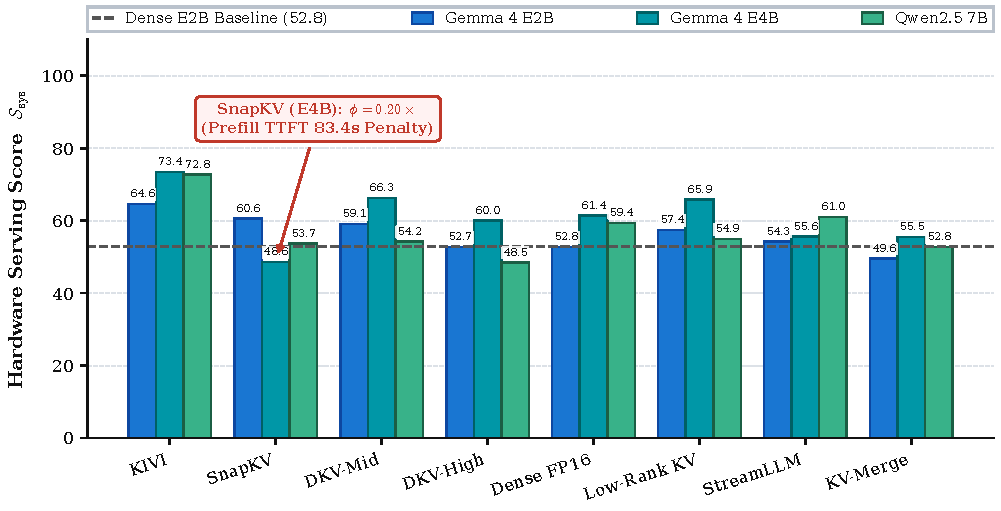
\includegraphics[width=0.92\textwidth]{figures/fig4_ssys_cross.pdf}
\caption{\textbf{Cross-Model Part 2 Hardware System Serving Utility Distribution.} Breakdown of $\mathcal{S}_{\text{sys}}$ across Gemma~4 E2B, Gemma~4 E4B, and Qwen2.5~7B.}
\label{fig:ssys_cross}
\end{figure}

\vspace{-4pt}
\begin{figure}[h]
\centering
\begin{minipage}[t]{0.485\textwidth}
\centering
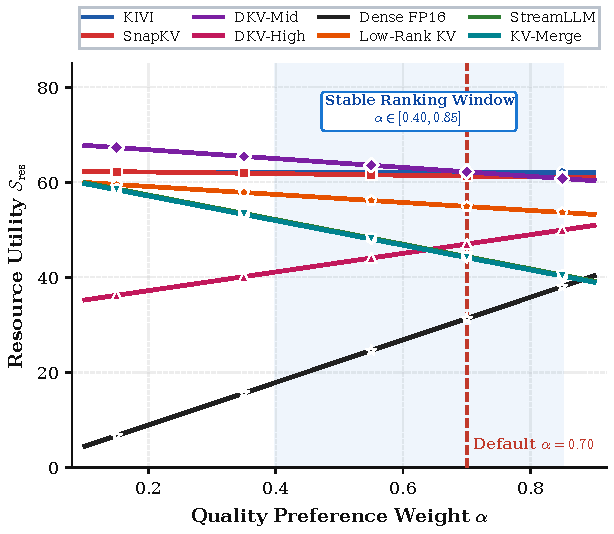
\includegraphics[width=\linewidth]{figures/fig8a_ranking_stability.pdf}
\caption{\textbf{Ranking Stability Across $\alpha$.} Trajectories across $\alpha \in [0.1, 0.9]$.}
\label{fig:alpha_stability}
\end{minipage}\hfill
\begin{minipage}[t]{0.485\textwidth}
\centering
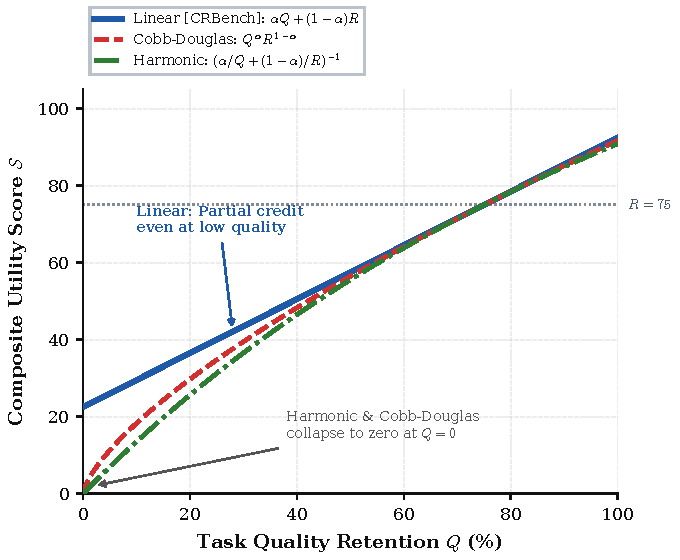
\includegraphics[width=\linewidth]{figures/fig8b_formulation_comparison.pdf}
\caption{\textbf{Utility Formulation Comparison.} Linear vs. Cobb--Douglas vs. Harmonic at $R_{\text{mem}} = 75\%$.}
\label{fig:formulation_comparison}
\end{minipage}
\end{figure}

\end{document}
